\documentclass{beamer}
\usepackage[ngerman]{babel}
\usepackage{booktabs}
\usepackage{tabulary}
\usepackage{siunitx}

\usetheme{imise}
\author{Konrad Höffner}
\date{2017-07-20, Abschlusstreffen}
\title{Meine persönlichen Erkenntnisse aus dem SNIK-Projekt}
\subtitle{Ontologiemodellierung und Entwicklung}
%{\url{https://github.com/KonradHoeffner/latex/releases/download/colloquium/colloquium.pdf}}
\newcommand{\todo}[1]{TODO: #1}
\newcommand{\imageslide}[3][]
{
\begin{frame}{#2}
\centering\includegraphics[width=1\textwidth,height=0.8\textheight,keepaspectratio]{#3}
\\#1
\end{frame}
%\usebackgroundtemplate{}
}

\AtBeginSection[]{
  \begin{frame}
  \vfill
  \centering
  \begin{beamercolorbox}[sep=8pt,center,shadow=false,rounded=true]{title}
    \usebeamerfont{title}\insertsectionhead\par%
  \end{beamercolorbox}
  \vfill
  \end{frame}
}

\begin{document}
\begin{frame}
\titlepage
\end{frame}

\section{OWL Restrictions}

\imageslide{Vorstellung}{img/virtual.png}
\imageslide{Erwartung}{img/virtual-expectation.png}

\begin{frame}{Lösung: OWL Restrictions}
\begin{itemize}
\item Modellierung durch OWL Restrictions
\item in existierender Protege-Datei vorhanden
\item Standardmechanismus für solche Fälle
\item erlaubt detaillierte Aussagen, z.B. someValuesFrom, allValuesFrom, cardinality restrictions,$\ldots$
\end{itemize}
\end{frame}

\begin{frame}{Problem}
\begin{itemize}
\item ständige Verwirrung bei Extraktion 
\item schwerer zu implementieren
\item Möglichkeiten nicht genutzt
\item 11600 restrictions, 11235 someValuesFrom, 189 allValuesFrom 176 andere 
\item Weiter verwenden oder abschaffen?
\end{itemize}
\end{frame}

\section{Ontologieplanung}

\imageslide[\url{http://www.snik.eu} \url{http://5stardata.info}]{Publizierung}{../sniktec/img/5star.png}

\section{Toolentwicklung}
\imageslide[\url{https://github.com/IMISE/snik-ontology}]{RDF Dump}{../sniktec/img/rdfdump.png}
\imageslide[\url{https://protegewiki.stanford.edu/}]{RDF Dump in Protégé}{../sniktec/img/protege.png}
\imageslide[\url{http://www.snik.eu/sparql}]{SPARQL Endpoint}{../sniktec/img/sparqlresult.png}

\imageslide[\url{http://www.snik.eu/ontology}]{RDF Browser---LodView}{../sniktec/img/browse-cio.png}

\imageslide[\url{http://www.snik.eu/graph}]{Graphvisualisierung I}{../sniktec/img/graph-entitytype.png}
\imageslide[\url{http://www.snik.eu/graph}]{Graphvisualisierung II}{../sniktec/img/graph-erf.png}

\begin{frame}{LodLive \& Relfinder}
\centering
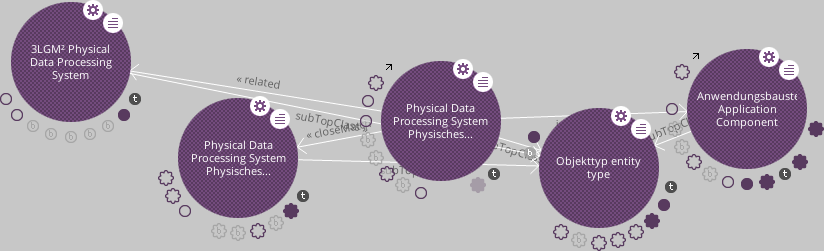
\includegraphics[width=\textwidth]{../sniktec/img/lodlive.png}\\
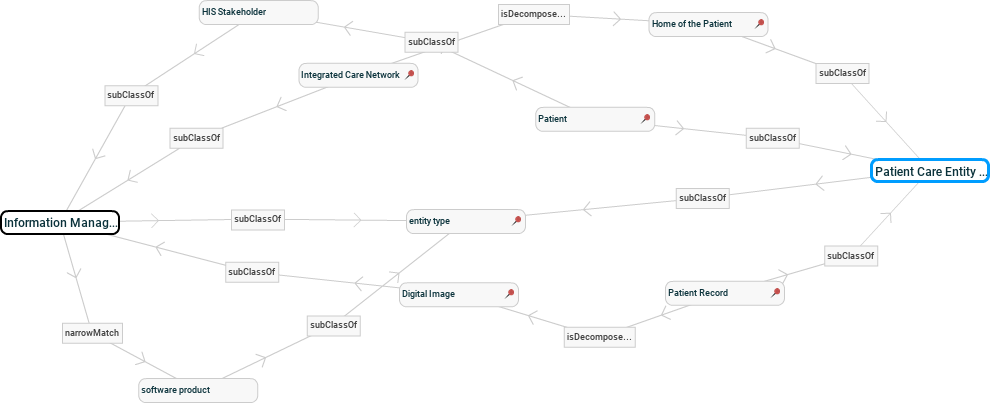
\includegraphics[width=\textwidth]{../sniktec/img/relfinder.png}
\end{frame}

\imageslide[https://imise.github.io/snik-ontology/2017/04/12/dashboard]{Statistiken}{../sniktec/img/dashboard-medley.png}
\imageslide[\url{https://github.com/IMISE/snik-ontology/issues}]{Ticketsystem}{../sniktec/img/gitissue.png}
\imageslide[\url{http://www.snik.eu/evaluation}]{TripleCheckMate}{../sniktec/img/triplecheckmate.png}

\imageslide[http://aksw.org/Projects/LIMES]{LIMES}{../sniktec/img/limes.png}

\imageslide[https://github.com/IMISE]{Öffentliche Softwarerepositories}{../sniktec/img/github.png}

\begin{frame}{Beobachtungen und Future Work}
\begin{itemize}
\item Verlust von Mitarbeitern und SHKs
\item gute Kooperation von Herr Smers mit Birgit und mir 
\item Feedbackkreislauf mit Lehre, Kooperationsprojekt 
\item Kooperation mit AKSW sehr hilfreich
\item Open Data in vielerlei Hinsicht positiv aber Vorsicht nötig
\item Rücksicht auf ältere Browser 
\end{itemize}
\end{frame}

\begin{frame}{Beobachtungen und Future Work}
\begin{itemize}
\item Evaluationsmöglichkeiten (TripleCheckMate) da aber wenig genutzt
\item Bekanntmachung versucht (Facebook, Twitter, Papers) aber mehr nötig
\item Visualisierung Priorität vor Journalpaper 
\item Ontologie nie fertig, schwere Priorisierung
\item Anordnung und Auswahl Visualisierung nach Zweck schwierig
\item großes Potential
\item Idealerweise viele Beschäftigungsmöglichkeiten: Programmieren, Testen, Social Media, UI, Krankenhaus-Instanzen$\ldots$
\end{itemize}
\end{frame}

\begin{frame}{Beobachtungen und Future Work}
\begin{itemize}
\item sehr angenehmes Arbeitsumfeld
\item schwieriges technisches Umfeld, große Hilfe durch Sebastian Stäubert
\item Doktorarbeit etwas in den Hintergrund gerutscht
\item sehr gute Kooperation
\item freue mich auf Elternzeit und auf danach Projekt zuende führen
\end{itemize}
\end{frame}

\end{document}
